\section{Coulomb-Nuclear Interference}
\label{sec:coulomb}

This section presents a study of the measured differential cross-section, where the Coulomb-nuclear interference (CNI) is used as a tool to probe the nuclear component of the scattering amplitude. Since the CNI effects are sensitive to the phase of the nuclear amplitude, both modulus and phase can be tested. For the modulus, a relevant question is whether the earlier reported non-exponentiality of differential cross-section \cite{8tev-90m} can be attributed solely to the nuclear component or whether Coulomb scattering gives an important contribution. Concerning the phase, several parametrisations with different physics interpretations will be tested and the phase value at $t = 0$ will be determined (as the $\rho$ parameter).

The presentation starts with Section~\ref{sec:cni framework} outlining the theoretical concepts needed to describe the CNI effects. It is followed by Section~\ref{sec:cni anal proc} providing details on fitting procedures used to analyse the data. Sections \ref{sec:fit exp1} and \ref{sec:fit exp3} discuss fit results for two relevant physics alternatives: purely exponential and non-exponential nuclear modulus.



%----------------------------------------------------------------------------------------------------

\subsection{Theoretical Framework}
\label{sec:cni framework}

The amplitude describing elastic scattering of protons may be expected to receive three contributions, each corresponding to one of the following Feynman diagram sets.
\begin{itemize}
\item Containing QED elements only. This amplitude can be calculated from first principles, see Section~\ref{sec:cni coulomb}.
\item Containing QCD elements only. This amplitude is not calculable from first principles, Sections~\ref{sec:cni nuclear modulus} and \ref{sec:cni nuclear phase} will propose several phenomenologically motived parametrisations.
\item Containing both QED and QCD elements. This contribution is neither calculable from first principles, neither ad hoc parametrisation can be used -- this amplitude is correlated with the previous two. Section~\ref{sec:cni interference} will introduce two interference formulae attempting to calculate corresponding effects.
\end{itemize}


%------------------------------------------------------------------
\subsubsection{Coulomb Amplitude}
\label{sec:cni coulomb}
%
The Coulomb amplitude can be calculated from QED (e.g.~Section 3.2 in \cite{block06}), using empirical electric ${\cal F}_{\rm E}$ and magnetic ${\cal F}_{\rm M}$ form factors of the proton. It can be shown (e.g.~Section 1.3.1 in~\cite{jan_thesis}) that, at low $|t|$, the effect of both form factors can be described by a single function ${\cal F}$:
\begin{equation}
\label{eq:coul cs}
	{\d\sigma^{\rm C}\over \d t} = {4\pi\alpha^2\over t^2}\,{\cal F}^4\ ,\qquad 
	{\cal F}^2 = {{\cal F}_{\rm E}^2 + \tau {\cal F}_{\rm M}^2\over 1 + \tau}\ ,\qquad 
	\tau = {|t|\over 4m^2}\ ,
\end{equation}
where $\alpha$ denotes the fine-structure constant and $m$ represents the proton mass.



%------------------------------------------------------------------
\subsubsection{Nuclear Amplitude -- Modulus}
\label{sec:cni nuclear modulus}

At $|t| \gtrsim 0.02\un{GeV^2}$ the effects due to the Coulomb interaction are not expected to be large (c.f.~Figure~\ref{fig:cni effect}). Thus, the measured cross-section can be -- to a large extent -- attributed to the nuclear component. Following Table~\ref{tab:data} and especially \cite{8tev-90m} which presents high-precision data for $|t| < 0.2\un{GeV^2}$, it is reasonable to parametrise the nuclear modulus as
\begin{equation}
\label{eq:nuc mod}
\left | {\cal A}^{\rm N}(t) \right | = \sqrt{s\over\pi} {p\over \hbar c} \sqrt{a} \exp\left( {1\over 2} \sum\limits_{n = 1}^{N_b} b_n\, t^n \right)\ ,
\end{equation}
where $N_b$ gives the number of free parameters in the exponent. Consistently with \cite{8tev-90m}, the parameter $b_1$ gives the forward diffractive slope and $a$ the intercept of the differential cross-section at $t=0$. This parametrisation is also compatible with a number of theoretical models (see e.g.~\cite{elegent}).

Since the calculation of CNI may, in principle, involve integrations (e.g.~Eq.~(\ref{eq:int kl})), it is necessary to extend the parametrisation meaningfully to $|t| > 0.2\un{GeV^2}$. Therefore, at $|t| > 0.5\un{GeV^2}$, the parametrisation is anchored to a preliminary cross-section derived from the same data set as in \cite{8tev-90m} which features a dip-bump structure similar to the one observed at $\sqrt{s} = 7\un{TeV}$ \cite{epl95}. The region $0.2 < |t| < 0.5\un{GeV^2}$ is reserved for a smooth transition between the parametrisation in Eq.~(\ref{eq:nuc mod}) and the anchored part. It will be shown that changing the high-$|t|$ part has negligible impact on the results presented later on.


%------------------------------------------------------------------
\subsubsection{Nuclear Amplitude -- Phase}
\label{sec:cni nuclear phase}

Since one of the goals is to determine the value of $\rho$, this parameter is shared by all the below proposed parametrisations.

\begin{figure*}
\begin{center}
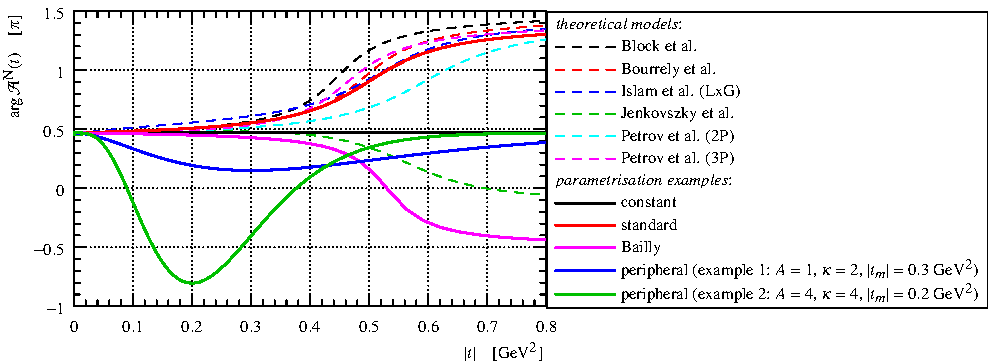
\includegraphics{fig/hadronic_phase_illustration.pdf}
\caption{Illustration of nuclear-phase forms. The dashed lines correspond to predictions by theoretical models (\cite{elegent} and references therein). The solid lines give typical examples of parametrisations used in this report, all at the same value of $\rho = 0.10$. The peripheral example corresponds to the parameter values in Eq.~(\ref{eq:nuc phase per val}).
}
\label{fig:phase illustration}
\end{center}
\end{figure*}


% ***
A {\bf constant phase} is obviously the simplest choice:
\begin{equation}
\label{eq:nuc phase con}
\arg {\cal A}^{\rm N}(t) = {\pi\over 2} - \arctan\rho = \hbox{const.}
\end{equation}
Note that this is equivalent to a strict proportionality of real and imaginary part of the amplitude at all $t$.

% ***
The {\bf standard phase} parametrisation,
\begin{equation}
\label{eqn:nuc phase std}
\arg {\cal A}^{\rm N}(t) = {\pi\over 2} - \arctan\rho + \arctan \left(\frac{|t|-|t_{0}|}{\tau}\right) -  \arctan \left(\frac{-|t_{0}|}{\tau}\right) \: ,
\end{equation}
implements the main features of many theoretical models -- almost imaginary amplitude in the forward direction ($\rho$ small) while almost purely real in the (first) diffraction dip. The parameters $t_0 = - 0.50\un{GeV^2}$ and $\tau = 0.1\un{GeV^2}$ have been chosen such that the shape is similar to a number of model predictions, see Figure~\ref{fig:phase illustration}.

% ***
Another parametrisation is by {\bf Bailly et al.}~\cite{bailly87}:
\begin{equation}
\label{eq:nuc phase bai}
	\arg {\cal A}^{\rm N}(t) = {\pi\over 2} - \arctan {\rho\over 1 - {t\over t_{\rm d}}}
	%\arg {\cal A}^{\rm N}(t) = \arctan \left[ {1\over\rho} \left(1 - {t\over t_{\rm d}} \right) \right]\ ,
\end{equation}
where $t_{\rm d} \approx -0.53\un{GeV^2}$ gives the position of the diffractive minimum at $8\un{TeV}$ (preliminary result derived from the $\beta^* = 90\un{m}$ data \cite{8tev-90m}). This phase has a behaviour qualitatively similar to the model of Jenkovszky et al., see Figure~\ref{fig:phase illustration}.

% ***
The {\bf peripheral phase} \cite{kl94} provides an alternative to the above descriptions since it may yield a very different picture in the impact-parameter space. As shown in Figure~\ref{fig:phase illustration}, the parametrisation
\begin{equation}
\label{eq:nuc phase per}
\arg {\cal A}^{\rm N}(t) = {\pi\over 2} - \arctan\rho - \zeta_1 \left(- {t\over 1\un{GeV^2}} \right)^\kappa \e^{\nu t}
\end{equation}
can have a rapid variation at low $|t|$, then peaks at $t = -\kappa / \nu$ and asymptotically returns to its value value at $t=0$. According to \cite{kl-8tev}, reasonable parameter values at $\sqrt s = 8\un{TeV}$ are
\begin{equation}
\label{eq:nuc phase per val}
	\zeta_1 = 800\ ,\qquad
	\kappa = 2.311\ ,\qquad
	\nu = 8.161\un{GeV^{-2}}\ .
\end{equation}

Figure~\ref{fig:phase illustration} presents a comparison of phase predictions by several models to typical examples of parametrisations proposed above.

It should be noted that the nuclear phase has a strong influence on the amplitude behaviour in the space of impact parameter $b$ (for detailed discussion see e.g.~Section 3 in~\cite{klk02}). A particularly decisive feature is the rate of phase variation at low $|t|$. Looking at Figure~\ref{fig:phase illustration} one can see that the constant, standard and Bailly phases are essentially flat at low $|t|$, thus leading to qualitatively similar pictures in the impact parameter space: elastic collisions more central (preferring lower values of $b$) than the inelastic ones. Conversely, the peripheral phase parametrisation can yield a description with the opposite hierarchy, which is argued to be more natural by some authors (e.g. Section~4 in~\cite{kl96}). An impact-parameter study of the presented data will be given at end of Section~\ref{sec:fit exp3}.

%------------------------------------------------------------------
\subsubsection{Coulomb-Nuclear Interference Formulae}
\label{sec:cni interference}

The {\bf simplified West-Yennie formula (SWY)} \cite{wy68} is derived in the framework of perturbative quantum field theory by evaluating the lowest-order Feynman diagrams that comprise both nuclear and Coulomb interactions. In this approach, the interference is reduced to an additional phase between the Coulomb and nuclear amplitudes. Moreover, several approximations were used in the derivation. First, in order to avoid integrating over off-mass-shell contributions to the nuclear amplitude (essentially unknown), very slow variation of the nuclear amplitude phase was assumed: $\arg {\cal A}^{\rm N} \approx \hbox{const}$. Then, in order to obtain a closed-form expression, the exponential slope of the nuclear modulus was assumed constant (i.e.~only $b_1$ non-zero in parametrisation Eq.~(\ref{eq:nuc mod})). The original formula did not contain the electromagnetic form factor ${\cal F}$, which was added later by hand:
\begin{equation}
\label{eq:int swy}
	{\d\sigma\over \d t}^{\rm C+N} = {\pi (\hbar c)^2 \over s p^2} \left | {\alpha s\over t} {\cal F}^2 \e^{\I\alpha \Phi(t)} + {\cal A}^{\rm N} \right |^2\ ,\qquad
	\Phi(t) = - \left( \log {b_1 |t|\over 2} + \gamma \right)\ ,
\end{equation}
where $\alpha$ is the fine-structure constant and $\gamma \doteq 0.577$ the Euler constant. Despite the many limitations, the formula has extensively been used in past data analyses. For backward-comparison reasons we consider it also in this report.

\begin{figure*}
\begin{center}
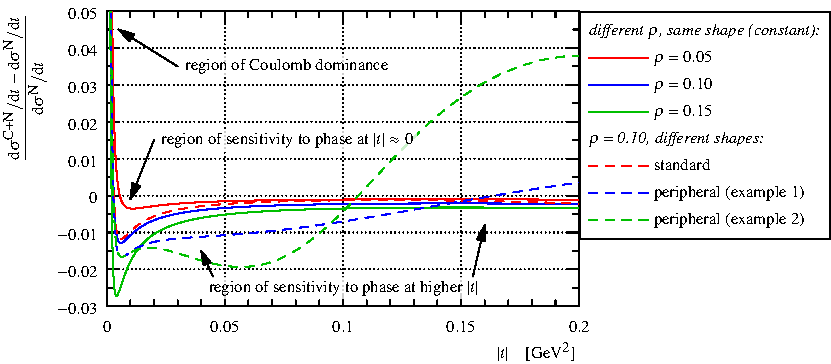
\includegraphics{fig/cni_effect_illustration.pdf}
\caption{%
Illustration of the effects due to the Coulomb interaction, using the KL formula. For the SWY formula, the picture is similar, however it misses the effects at $|t| \gtrsim 0.02\un{GeV^2}$. The curves show a response of the interference formula to different nuclear phases with a purely exponential nuclear modulus. The solid curves correspond to phases of the same shape (constant) but different values of $\rho$: the maximal response can be seen at $|t| \lesssim 0.01\un{GeV^2}$. Conversely, the dashed lines correspond to phases with fixed $\rho$ but various shapes (the same examples as in Figure~\ref{fig:phase illustration}): response sizeable at $|t| \gtrsim 0.02\un{GeV^2}$.
}
\label{fig:cni effect}
\end{center}
\end{figure*}

The {\bf Kundr\' at-Lokaj\' i\v cek formula (KL)} \cite{kl94} was derived in an impact parameter formalism and is based on the additivity of eikonals. The derivation poses no limitations on the nuclear amplitude, and the formula naturally incorporates the electromagnetic form factor. In this treatment, the interference effect goes beyond a single phase, the $G$ quantity is complex, in general:\footnote{%
Note that many recent publications by the same authors contain a misprint: wrong sign in front of the second term contributing to $G(t)$.
}
\begin{equation}
\label{eq:int kl}
	\begin{aligned}
		{\d\sigma\over \d t}^{\rm C+N} &= {\pi (\hbar c)^2 \over s p^2} \left | {\alpha s\over t} {\cal F}^2
			+ {\cal A}^{\rm N}\, \Big[1 - \I\alpha G(t)\Big] \right |^2\ ,\cr
		G(t) &= 
			\int \d t'\, \log {t'\over t} {\d\phantom{t'}\over \d t'} {\cal F}^2(t')
			- \int \d t' \left( {{\cal A}^{\rm N}(t') \over {\cal A}^{\rm N}(t)} - 1 \right) { I(t, t')\over 2\pi }
			\ ,\cr
		I(t, t') &= \int_0^{2\pi} \d\phi\ {{\cal F}^2(t'')\over t''}\ ,\qquad t'' = t + t' + 2\sqrt{t\, t'} \cos\phi\ ,\cr
	\end{aligned}
\end{equation}
where the $t$ integrations extend over the entire kinematically allowed region. A slightly different variant proposed in Eq.~(22) in~\cite{kl05} was considered, too:
\begin{equation}
\label{eq:int kl exp}
	{\d\sigma\over \d t}^{\rm C+N} = {\pi (\hbar c)^2 \over s p^2} \left | {\alpha s\over t} {\cal F}^2
		+ {\cal A}^{\rm N}\, \e^{- \I\alpha G(t)} \right |^2 \ .
\end{equation}

By analysing the formulae Eq.~(\ref{eq:int swy}) and (\ref{eq:int kl}), one can conclude that in the region where the nuclear amplitude dominates ($|t| \gtrsim 0.003\un{GeV^2}$), the effects due to the Coulomb interaction are of the order of $\alpha$ or the ratio ${\cal A}^{\rm C} / {\cal A}^{\rm N}$. In both cases, the magnitude of the interference effects can be expected at a percent level, as shown in Figure~\ref{fig:cni effect}. The figure also shows that the effects at different $|t|$ probe different parts of the nuclear phase: maximum sensitivity to $\rho$ lies at very low $|t|$ while at higher $|t|$ the effects are sensitive to phase values at slightly higher $|t|$. It can also be observed that for the constant, standard and Bailly phase the effects are very similar and rather mild at higher $|t|$. This can be understood from a very limited variation of the phase at low $|t|$, which is the region contributing most to the integral in Eq.~(\ref{eq:int kl}). On the contrary, the higher $|t|$ response to peripheral phases can have various forms, often similar to the ``U shape'' of the reconstructed cross-section, see the top plots in Figures~\ref{fig:fit exp1} and~\ref{fig:fit exp3}.


%----------------------------------------------------------------------------------------------------
\subsection{Analysis Procedure}
\label{sec:cni anal proc}

Beyond using the data from Table~\ref{tab:data}, one might consider including $\beta^* = 90\un{m}$ data \cite{8tev-90m} which benefit from much smaller uncertainties. However, due to the limited reach, $|t| \gtrsim 0.03\un{GeV^2}$, they have essentially no sensitivity to the $\rho$ parameter, cf.~Fig.~\ref{fig:cni effect}. Furthermore, due to possible systematic tensions between the data sets, inclusion of the $\beta^* = 90\un{m}$ data may have deteriorating impact on the $\rho$ determination. Therefore, the value of $\rho$ was determined from $\beta^* = 1000\un{m}$ data only. For other parameters to which both data sets have non-negligible sensitivity (e.g.~$b_i$ in Eq.~(\ref{eq:nuc mod})), both data sets should give compatible results. This has been verified for all the fits presented later on. Since the $\beta^* = 90\un{m}$ data yield much lower uncertainties, both data sets have been used for determining all parameters except $\rho$. In practice, a series of two fits was performed:
\begin{enumerate}[leftmargin=2cm]
\item[step 1:] fit of $\beta^* = 1000\un{m}$ data with $\rho$ free,
\item[step 2:] fit of $\beta^* = 1000$ and $90\un{m}$ data with $\rho$ fixed from the preceding step.
\end{enumerate}

Each of the fits has been performed according to the standard least-squares method, however with the following two different implementations.

\begin{enumerate}

% ***
\item[A.] This approach consists of minimising
\begin{equation}
\label{eq:chi sq A}
	\chi^2 = \Delta^\T \mat V^{-1} \Delta\ ,\qquad
	\Delta_i = \left.{\d\sigma\over \d t}\right|_{{\rm bin}\ i} - {\d\sigma^{\rm C+N}\over\d t}\left(t^{\rm rep}_{{\rm bin}\ i}\right)\ ,\qquad
	\mat V = \mat V_{\rm stat} + \mat V_{\rm syst}\ ,
\end{equation}
where $\Delta$ is a vector of differences between the differential cross-section data and a fit function $\d\sigma^{C+N}/\d t$ evaluated at representative points $t^{\rm rep}$ of each bin \cite{lafferty94}. The minimisation is repeated several times, and the representative points are updated between iterations. The CNI effects are calculated using the computer code from~\cite{elegent}. The covariance matrix $\mat V$ is composed of two components. The diagonal of $\mat V_{\rm stat}$ contains the statistical uncertainty squared from Table~\ref{tab:data} and from Table~3 in \cite{8tev-90m}. $\mat V_{\rm syst}$ includes all systematic uncertainty contributions except the normalisation, see Eq.~(\ref{eq:covar mat}) and Eq.~(14) in \cite{8tev-90m}. For improved fit stability, the normalisation uncertainty is not included in the $\chi^2$ definition. Instead, the uncertainty is propagated for each fit parameter. For this purpose, the fit is repeated with $-1\un{\sigma}$, $0\un{\sigma}$ and $+1\un{\sigma}$ biases independently in: global normalisation ($1\un{\sigma} = 4.2\un{\%}$), $90\un{m}$ data normalisation ($0.08\un{\%}$) and $1000\un{m}$ data normalisation ($0.25\un{\%}$). This gives a sample of 27 fit results, from which one can estimate the propagated normalisation uncertainty of a parameter as $(\hbox{max} - \hbox{min})/2$, where ``max'' (``min'') is the greatest (smallest) value in the sample. This normalisation uncertainty is, at the end, added quadratically to the uncertainty reported by the fit with no bias.


% ***
\item[B.] \TODO{Hubert's approach}
\iffalse
\begin{equation}
\label{eq:chi sq B}
	\chi^2 = \Delta^\T \mat V^{-1} \Delta + ...\ ,\qquad
	\Delta_i = \left.{\d\sigma\over \d t}\right|_{{\rm bin}\ i} - {1\over \Delta t_i} \int_{{\rm bin}\ i} f(t)\,\d t\ ,\qquad
	\mat V = \mat V_{\rm stat} + \mat V_{\rm syst}\ ,
\end{equation}
$\Delta t_i$ representing the width of the $i$-th bin. Custom implementation of interference formulae?
\fi

\end{enumerate}


The fits have shown extremely low sensitivity to a number of the above presented choices, summarised in the following list. 
\begin{itemize}
\item Choice of the form factor in Eq.~(\ref{eq:coul cs}). The options considered in \cite{elegent} have been tested, none of them giving any significant difference with respect to the default choice \cite{puckett10}.
\item Extension of the nuclear modulus to non-measured $|t|$ region, see last paragraph in Section~\ref{sec:cni nuclear modulus}. No effect was observed when the high-$|t|$ part was altered (both shape and normalisation) nor when the size of the transition region was changed.
\item The two variants of the KL formula, Eqs.~(\ref{eq:int kl}) and (\ref{eq:int kl exp}).
\item Fit implementations A and B, manifesting the stability of the fit results.
\item Fits with constant, standard and Bailly phase are practically indistinguishable. This can be expected from Fig.~\ref{fig:cni effect} showing that the corresponding CNI effects are very similar. Therefore, later on these phases will be treated as one family represented by the constant phase.
\end{itemize}


As anticipated above, one of the goals of this study is to probe the origin of the earlier observed differential cross-section non-exponentiality \cite{8tev-90m}. Therefore, the following two classes of fits were considered.
\begin{itemize}
\item Section \ref{sec:fit exp1}: fits with purely-exponential nuclear modulus, that is $N_b=1$ in Eq.~(\ref{eq:nuc mod}). In this case, the non-exponentiality must come from the CNI effects.
\item Section \ref{sec:fit exp3}: fits with nuclear modulus flexible enough to describe the non-exponentiality without the CNI effects. Here, the non-exponentiality may be due to the nuclear modulus, CNI effects or both.
\end{itemize}
For each of these nuclear modulus cases, the following two phase parametrisation were considered:
\begin{itemize}\setlength\itemsep{0pt}
\item constant phase, Eq.~(\ref{eq:nuc phase con}), as a representative of the central-phases family,
\item peripheral phase, Eq.~(\ref{eq:nuc phase per}) with parameters fixed to the values in Eq.~(\ref{eq:nuc phase per val}) to represent peripheral behaviour in the impact parameter space.
\end{itemize}

The results of any fit can be used to calculate the total cross-section via the optical theorem:
\begin{equation}
\label{eq:si tot}
\sigma_{\rm tot}^2 = {16\pi\, (\hbar c)^2\over 1 + \rho^2}\, a\ .
\end{equation}
Note that unlike all previous LHC analyses, in this report all the ingredients are obtained consistently from the same source.


%----------------------------------------------------------------------------------------------------
\subsection{Fits with Purely-Exponential Nuclear Modulus}
\label{sec:fit exp1}

The goal of this section is to test whether the data are compatible with purely-exponential nuclear modulus, i.e.~$N_b=1$ in Eq.~(\ref{eq:nuc mod}). In other words, the non-exponentiality is forced to originate in the Coulomb-induced effects. The fit results obtained with KL and SWY (where applicable) formulae are summarised in Table~\ref{tab:fit exp1} and shown in Fig.~\ref{fig:fit exp1}.

\begin{table}
\caption{Fit results with $N_b=1$. Each column corresponds to a fit with different interference formula and/or nuclear phase.}
\vskip-3mm
\label{tab:fit exp1}
\begin{center}
\setlength\tabcolsep{2.5mm}
\small
\input fig/fit_exp1/table_data.tex
\end{center}
\end{table}

\begin{figure*}
\begin{center}
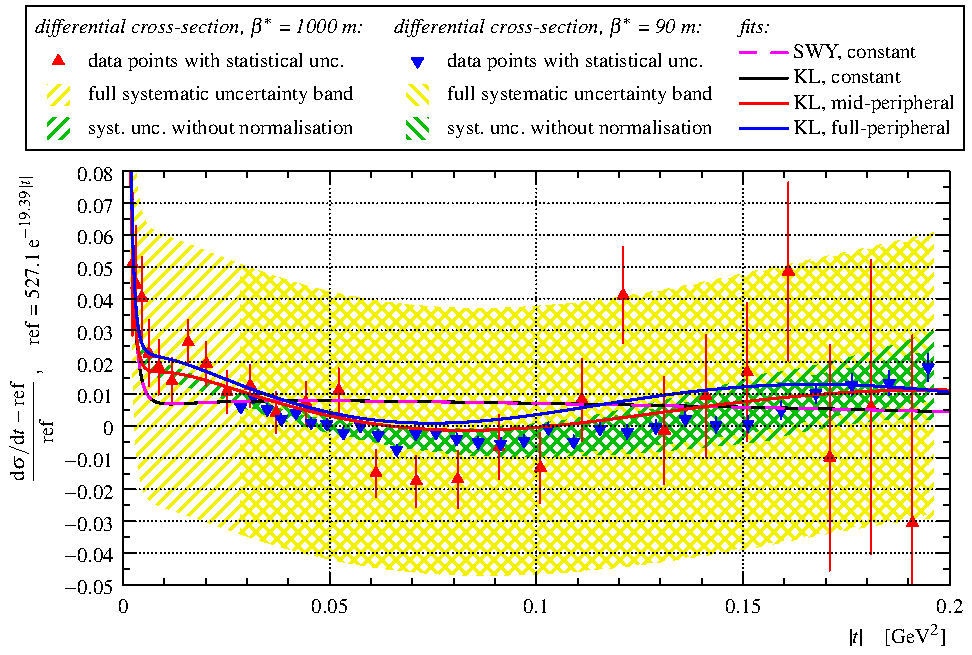
\includegraphics{fig/fit_exp1/t_dist_rel_with_fit.pdf}
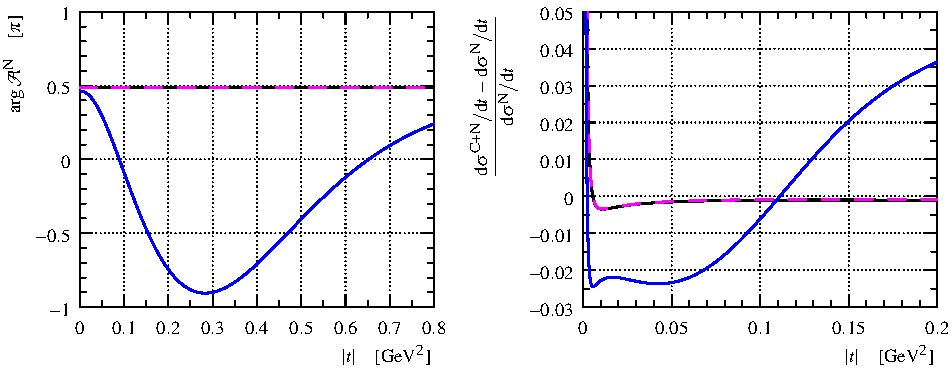
\includegraphics{fig/fit_exp1/phase_cni_effect.pdf}
\caption{Visualisation of fit results from Table~\ref{tab:fit exp1} obtained with $N_b=1$. The continuous (dashed) lines correspond to fits with KL (SWY) formula. Note that the fits with constant nuclear phase largely overlap.
TOP: fits compared to differential cross-section data in a relative reference frame, see the vertical axis label. The reference is identical to the one in \cite{8tev-90m}. 
BOTTOM LEFT: $t$-dependence of the nuclear phase as extracted from the fits.
BOTTOM RIGHT: the effects induced by the Coulomb interaction for each of the fits.
}%
\label{fig:fit exp1}
\end{center}
\end{figure*}

Table~\ref{tab:fit exp1} shows that both fits with constant phase are essentially identical and have bad fit quality. The step-2 fit using both $\beta^*=1000$ and $90\un{m}$ data can be excluded with $7.6\un{\sigma}$ significance. Consequently, since the combination of $N_b=1$ and constant phase is the only compatible with the SWY formula, its application is excluded, too.


Although the quality of the fit with the peripheral phase is good, this option seems disfavoured from different perspectives.
\begin{itemize}
\item There are several theoretical reasons for the nuclear component being non-exponential, e.g.~\cite{kmr00-multiPom,kmr12-opacity,kmr15-slope}. Indeed, most elastic scattering models predict non-exponential nuclear modulus, see e.g.~\cite{elegent}.
\item The value of $\rho$ obtained in this fit constitutes an outlier with respect to a consistent pattern of other fits from this report and extrapolations from lower energies: e.g.~\cite{fagundes11,block12,compete} and most models in \cite{elegent}.
\end{itemize}
Let us also recall that the good quality of this fit is possible due to the more complex KL formula where the CNI effects go beyond an additional phase in the traditional SWY concept.


%----------------------------------------------------------------------------------------------------
\subsection{Fits with Non-Exponential Nuclear Modulus}
\label{sec:fit exp3}

The aim of this section is to discuss fits with enough flexibility in the nuclear modulus to describe the non-exponentiality in the data. For this, $N_b=2$ to $5$ were considered. The optimal degree was chosen according to two criteria: reasonable $\chi^2/\hbox{ndf}$ and stability of fit parameters (among which $\rho$ is one of the most sensitive). For instance, with constant phase the fit (step 1) with $N_b=2$ yields $\chi^2/\hbox{ndf} = 1.07$ and $\rho = 0.10$ while with $N_b=3$ gives $\chi^2/\hbox{ndf} = 1.03$ and $\rho = 0.12$. Both fits have the normalised $\chi^2$ reasonably close to $1$, but the value of $\rho$ changes significantly between $N_b=2$ and $3$ which is unexpected should $N_b=2$ be sufficient. On the other hand $N_b=4$ gives $\chi^2/\hbox{ndf} = 0.861$ which is unreasonably low. Therefore $N_b=3$ was chosen.

\iffalse
* KL, exp2, con
\rh       =   0.101 \pm  0.026
last fit     : chi^2/ndf = 68.45/57 = 1.201, probability = 1.42E-01, significance = 1.467, quality = 0.000000
previous fit : chi^2/ndf = 27.74/26 = 1.067, probability = 3.71E-01, significance = 0.894

* KL, exp3, con
\rh       =   0.121 \pm  0.029
last fit     : chi^2/ndf = 57.59/56 = 1.028, probability = 4.16E-01, significance = 0.813, quality = 0.000000
previous fit : chi^2/ndf = 25.63/25 = 1.025, probability = 4.27E-01, significance = 0.794

* KL, exp4, con
rho    =   0.087 +-  0.034
last fit     : chi^2/ndf = 54.48/55 = 0.990, probability = 4.95E-01, significance = 0.683, quality = 0.000000
previous fit : chi^2/ndf = 20.66/24 = 0.861, probability = 6.59E-01, significance = 0.442
\fi

Since non-exponential hadronic modulus is used, the only applicable interference formula is KL.

As shown in Table~\ref{tab:fit exp3}, both fits yield very reasonable fit quality and remarkably consistent values of $\rho$ (identical within the resolution) which are compared to previous measurements in Fig.~\ref{fig:rho cmp exp3}.

Fig.~\ref{fig:fit exp3} shows that the level of Coulomb-induced effects is very different in the fits. It is much stronger in the peripheral-phase case which can be expected as the phase features faster variation in the low-$|t|$ region.


\begin{table}
\caption{Fit results with KL formula and $N_b=3$.}
\vskip-3mm
\label{tab:fit exp3}
\begin{center}
\setlength\tabcolsep{5mm}
\small
\input fig/fit_exp3/table_data.tex
\end{center}
\end{table}

\begin{figure*}
\begin{center}
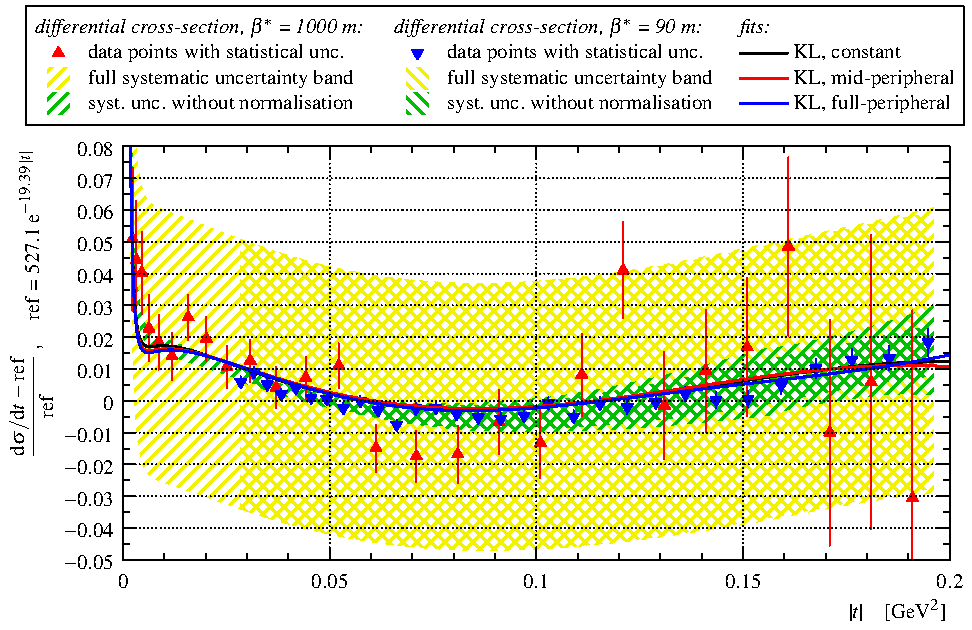
\includegraphics{fig/fit_exp3/t_dist_rel_with_fit.pdf}
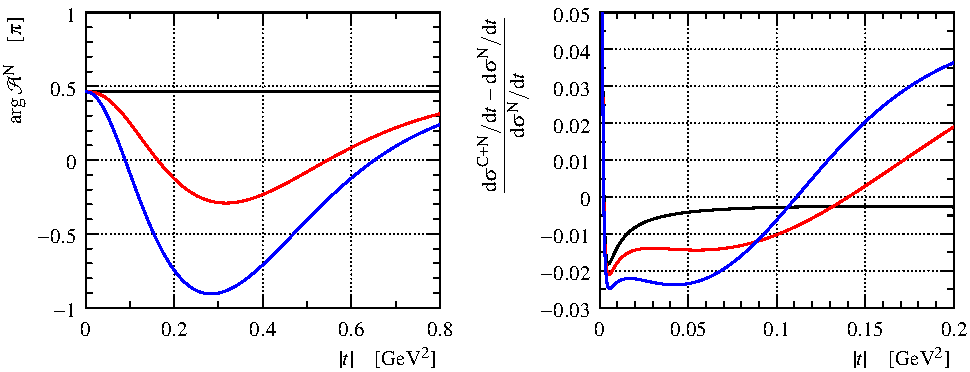
\includegraphics{fig/fit_exp3/phase_cni_effect.pdf}
\caption{Visualisation of fit results from Table~\ref{tab:fit exp3} obtained with KL formula and $N_b=3$. The solid lines correspond to fits with different nuclear phases.
TOP: fits compared to differential cross-section data in a relative reference frame, see the vertical axis label. The reference is identical to the one in \cite{8tev-90m}. 
BOTTOM LEFT: $t$-dependence of the nuclear phase as extracted from the fits.
BOTTOM RIGHT: the effects induced by the Coulomb interaction for each of the fits.
}%
\label{fig:fit exp3}
\end{center}
\end{figure*}


\begin{figure*}
\begin{center}
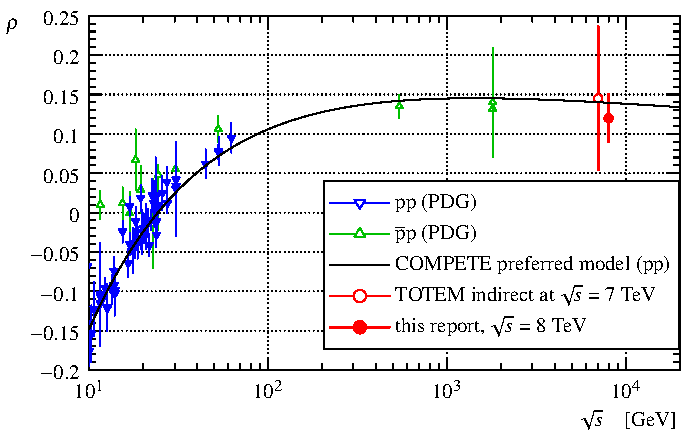
\includegraphics{fig/rho_s.pdf}
\caption{Energy dependence of the $\rho$ parameter. The blue (green) triangles correspond to $\rm pp$ ($\rm \bar pp$) data from PDG \cite{pdg} -- note that most of these points were determined with the help of the SWY formula, shown inconsistent with the presented data. The hollow red dot stands for the earlier indirect determination by TOTEM \cite{epl101-tot}. The full red dot represents the two results from Table~\ref{tab:fit exp3} which are numerically identical within the resolution. The black curve gives the preferred $\rm pp$ model by COMPETE \cite{compete}, obtained without using LHC data.
}%
\label{fig:rho cmp exp3}
\end{center}
\end{figure*}


The total cross-section results from the two fits in Table~\ref{tab:fit exp3} are well consistent with each other and also with previous measurements \cite{8tev-90m,epl101-el}. The slightly higher values with respect to previous analyses neglecting the Coulomb interaction are expectable as long as $\rho > 0$. This leads to negative interference at low $|t|$ which, when separated, leads to an increase of nuclear cross-section intercept $a$ and thus also total cross-section via Eq.~(\ref{eq:si tot}).


It is interesting to study the fit behaviour in the impact-parameter space. The scattering amplitude in this representation (often called profile function), ${\cal P}(b)$, can be obtained from the nuclear amplitude by means of Fourrier-Bessel transform (see e.g.~\cite{klk02}):
\begin{equation}
\label{eq:prof fun}
	{\cal P}(b) = {1\over 4 p \sqrt s} \int\limits_{-\infty}^0 \d t\,J_0(b\sqrt{-t})\,{\cal A}^{\rm N}(t)\ .
\end{equation}
The profile functions for the two fits from Table~\ref{tab:fit exp3} are shown in Figure~\ref{fig:bdist exp3}. The fit with constant nuclear phase gives a distribution peaked at $b=0$. It corresponds to a behaviour which is more central that for the fit with peripheral phase, where the most frequent impact parameter value is $b\approx 1.2\un{fm}$. This observation can be generalised to non-elastic channels, too. Following Section~3 in \cite{klk02}, one can calculate mean values of $b^2$ for elastic ($\langle b^2\rangle_{\rm el}$), inelastic ($\langle b^2\rangle_{\rm inel}$) or all ($\langle b^2\rangle_{\rm tot}$) collisions:
\begin{equation}
\label{eq:ms b}
	\langle b^2\rangle_j = {
		\int b\,\d b\,b^2\, h_j(b)
		\over
		\int b\,\d b\, h_j(b)
	}\ ,\ 
	h_{\rm el}(b) = |{\cal P}(b)|^2\ ,\ 
	h_{\rm tot}(b) = \Im {\cal P}(b)\ ,\ 
	h_{\rm inel}(b) = h_{\rm tot}(b) - h_{\rm el}(b)\ .
\end{equation}
Their values in Figure~\ref{fig:bdist exp3} indicate that the fit with constant nuclear phase leads to a picture with elastic collisions more central than the inelastic ones. The hierarchy is inverted for the fit with peripheral phase.



\begin{figure*}
\begin{center}
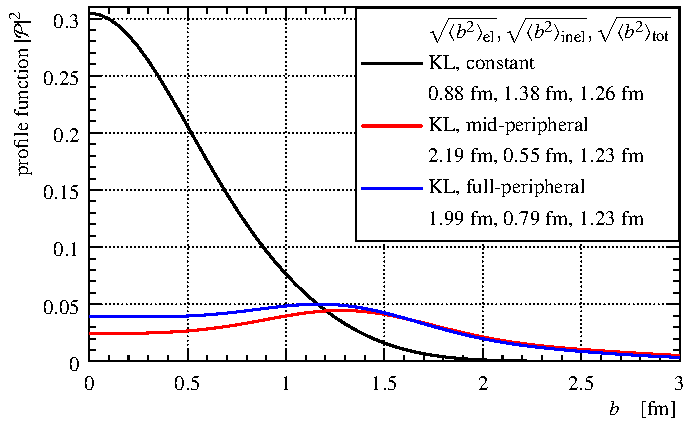
\includegraphics{fig/fit_exp3/b_dist.pdf}
\caption{%
Squared amplitude of the profile function, ${\cal P}$, as a function of impact parameter, $b$. The two lines correspond to the fits in Table~\ref{tab:fit exp3}, using the same colour code as in Figure~\ref{fig:fit exp3}. The root-mean-squares of $b$ in the legend are calculated from Eq.~(\ref{eq:ms b}).
}%
\label{fig:bdist exp3}
\end{center}
\end{figure*}


